%!TEX root = ../thesis.tex
%*******************************************************************************
%****************************** Third Chapter **********************************
%*******************************************************************************
\chapter{Results}

% **************************** Define Graphics Path **************************
\ifpdf
    \graphicspath{{Chapter3/Figs/Raster/}{Chapter3/Figs/PDF/}{Chapter3/Figs/}{Figs}}
\else
    \graphicspath{{Chapter3/Figs/Vector/}{Chapter3/Figs/}{Figs}}
\fi

\section{Mathematical model predicts different dynamical behaviours}
\label{sec:general_diff_behaviours}
% a weird name because before I used the term "general model" to contrast
% any sigB specific model. However, later on only the "general model" is
% discussed in the thesis

% Gillespie show diverse behaviours. why Gillespie
To validate the mathematical model which is based on the biochemical processes
(Section~\ref{sec:low_CN}), I simulated the time evolution of the system 
using the Gillespie algorithm (i.e. stochastic simulation algorithm) 
\cite{gillespie77}.
Previous work shows that a similar model simulated by the chemical Langevin 
equation (CLE) exhibits diverse dynamical behaviours (unpublished work by
Torkel Loman).
% The argument that CLE is not appropriate for the simulation
% is rather long. Might want to move this to Methods
However, CLE only holds on the condition that, in a time step,
the expected occurrence of the reaction is large enough and the change
of reaction rate is small enough, both of which are facilitated by a large
number of molecules present in the system \cite{gillespie00}.
Since the simulation focuses on dynamical behaviours such as stochastic pulsing
and stochastic switching between activation and inactivation
where low-copy number is important,
these assumptions may be violated.
The Gillespie algorithm generates statistically correct trajectories
from the chemical master equations \cite{gillespie77}, 
which is important for the low-copy number
regime here and also for establishing the bistability
in Section~\ref{sec:both_non_coop_bistability} which exploits
single-molecule dynamics.

% What are the types of behaviours and where to find them
Simulated with the Gillespie algorithm,
the model (Section~\ref{sec:low_CN}) 
displays a wide range of dynamical behaviours
when changing the activating and repressive forces
(Figure~\ref{fig:different_behaviours}).
% what are activating and repressive force?
% (why I talked about K_S and K_D first? because I'll talk about
% behaviour mapping next, and the parameters link the two)
% may be don't mention threshold here?
The parameters that tune the strength of activating and repressive forces 
are $K_S$ and $K_D$, respectively.
The activating force is inversely scaled by $K_S$ and, thus,
$K_S$ is called the activation threshold (which makes sense
especially in an ultrasensitive system).
Similarly, the repressive force is inversely scaled by $K_D$,
which serves as the repression threshold
(biochemical significance see Table~\ref{tab:general_model_paras}).
% Introduce the behaviour mapping
Seven primary types of dynamical behaviours emerge from
this simulation of an ultrasensitive (Hill coefficient $n = 3$)
sigma factor circuit.
To illustrate how the strength of activating and repressive 
forces determine the type of dynamical behaviours, I mapped
the behaviours to the parametric space of $K_S$ and $K_D$,
where the different behaviours are colour-coded
(Figure~\ref{fig:different_behaviours} centre).
% A list of dynamical behaviours
The seven types of dynamical behaviours are:

\begin{enumerate}[label=(\alph*)]
    \item No expression.
    \item Stochastic pulsing, characterized by the dominance of OFF-states
    interspersed with narrow peaks of expression.
    \item Oscillation, characterized by approximately periodic switching
    between ON and OFF states.
    \item Stochastic anti-pulsing, characterized by the dominance of 
    ON-states with stochastically timed transient shutdowns.
    \item Homogeneous activation, characterized by immediate activation
    upon exposure to stress.
    \item Stochastic switching, characterized by stochastically timed
    switching between ON- and OFF-states.
    \item Heterogeneous activation, characterized by heterogeneously
    delayed activation.
\end{enumerate}

% One more behaviour
And (h) irregular fluctuation, which typically exists
in non-ultrasensitive ($n = 1$) regime.
It is an intermediate dynamical behaviour between
stochastic pulsing and activation (more discussed in
Section~\ref{sec:us_for_bs_and_oscillation}).
A short trajectory along time for each behaviour is shown
in Figure~\ref{fig:different_behaviours}.
% Areas of pulsing and activation are large
% I may inferred too far here...
The behaviour mapping in Figure~\ref{fig:different_behaviours}
shows a wide range for stochastic pulsing (yellow) and 
homogeneous activation (deep blue), suggesting that these behaviours are
robust to the biochemical parameters and thus are more likely to be
conserved through neutral selection.
% separation by K_D/K_S
% this becomes a wordy paragraph, may suits discussion
% but can (somewhat floppily) used to argue that K_D/K_S and K_S 
% independently tune the system
Certain values of the ratio $K_D/K_S$ separates dynamical behaviours
(e.g. the vertical boundary of oscillation in 
Figure~\ref{fig:different_behaviours}).
This can be understood by rewriting the Hill term from Eq.~\ref{eqn:v_hill_2}
as:

\begin{align}
    v_H =& \frac{\sigma^n}{\sigma^n + 
        \left[A/\left(\frac{K_D}{K_S}\right) + K_S\right]^n}\\
    \approx& \frac{\sigma^n}{\sigma^n + 
        \left[A/\left(\frac{K_D}{K_S}\right)\right]^n}
\end{align}

Where $v_H$ is determined by the ratio $K_D/K_S$ and
notice that $v_H$ is the decisive factor for the expression rate of both
the sigma and anti-sigma factor.
The approximation holds when it satisfies $A/(\frac{K_D}{K_S}) >> K_S$,
as is often the case since most of the dynamical behaviours
happen when $K_D/K_S$ is around 1 and $K_S$ is small,
and when the circuit is activated, the abundance of the anti-sigma factor
is often dozens to hundreds.
% Now argue that increasing K_S (absolute value) promotes bistability
The absolute value of $K_S$ or $K_D$ is connected with whether the
system being bistable.
When $K_D/K_S$ is approximately greater than 1, as $K_S$ increases,
the dynamics transitions from monostability (including stochastic
anti-pulsing and homogeneous activation) to bistability (including
stochastic switching and heterogeneous activation)
(Figure~\ref{fig:different_behaviours}).
In bistable dynamics, state-flipping is triggered by stochastic
fluctuations \cite{eldar10a}.
Thus, as the activation threshold $K_S$ (or repression
threshold $K_D$) increases, the event of noise break-through becomes
more rare and tends to lock the circuit in one of the states,
which explains the transition from monostability to bistability.
% summary: independent turing by K_D/K_S and K_S
In summary, the behaviour mapping (Figure~\ref{fig:different_behaviours}
centre) can be roughly understood by independently tuning
bistability/monostability by $K_S$ and the relative activating
force by $K_D/K_S$.

% Experimental confirmation
The significance of the dynamical behaviours predicted by
the model is supported by experiments.
Single-cell measurements of the activation of $\sigma^B$ in
\textit{B. subtilis} shows stochastic pulsing \cite{locke11,cabeen17},
while the heterogeneous activation delay is observed in
\textit{B. subtilis} $\sigma^V$ dynamics \cite{schwall21a}.

\begin{figure}[ht]
    \centering
    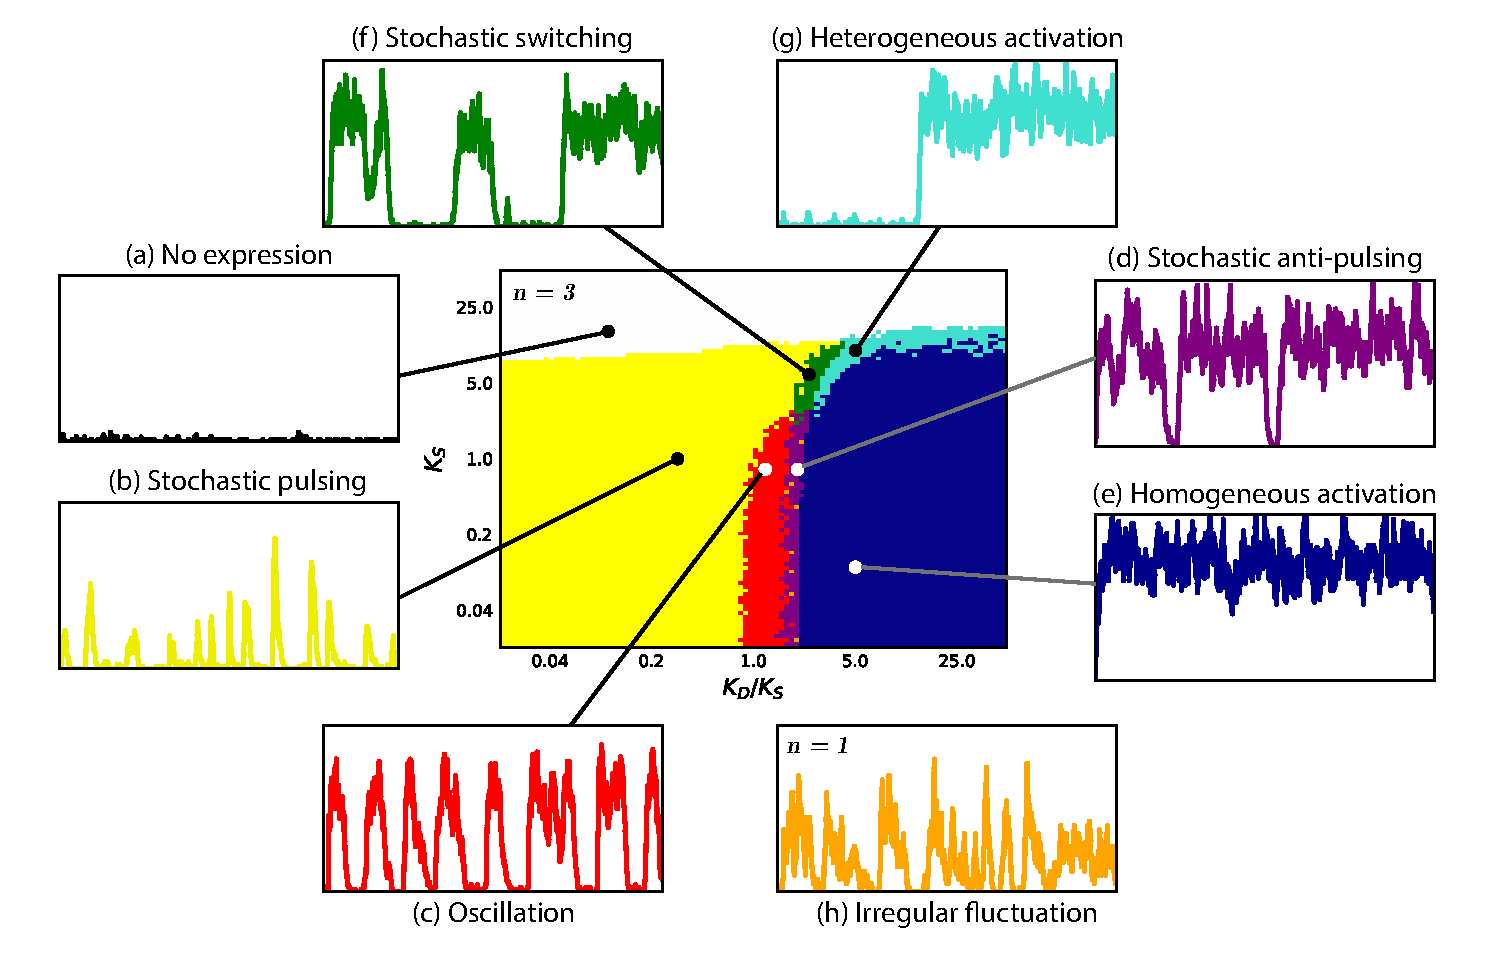
\includegraphics[width = 6in]{different_behaviours.pdf}
    \caption[
        Different dynamical behaviours generated by the mathematical
        model and their mapping to the parametric space
        ]{
        \textbf{Different dynamical behaviours generated by the mathematical
        model and their mapping to the parametric space.}
        (a-g) shows the time-trajectory (x-axis: time and y-axis:
        the amount of sigma factors) of the types of behaviours.
        The trajectory starts immediately after exposure to stress.
        (middle) the types of behaviours mapped to a 
        $K_S$-$K_D/K_S$ parametric space,
        simulated under ultrasensitive Hill coefficient $n = 3$.
    }
    \label{fig:different_behaviours}
\end{figure}

\subsection{Ultrasensitivity is important for bistability and oscillation}
\label{sec:us_for_bs_and_oscillation}

% bistability and oscillations are lost in non-ultrasensitivity
% "ultrasensitivity of the circuit" emphasizes intrinsic ultrasensitivity
To ask what role ultrasensitivity of the circuit plays in its dynamics,
I simulated the range of behaviours across the $K_S$-$K_D/K_S$ 
parametric space with either $n = 1$ (non-ultrasensitive) or
$n > 1$ (ultrasensitive).
%%
The loss of ultrasensitivity significantly changes the landscape
of the behaviour mapping,
with the stochastic anti-pulsing region much expanded and
the oscillation and heterogeneous activation
region completely lost (Figure~\ref{fig:behaviour_mappings_diff_n} A).
%%
A dynamical behaviour is considered stochastic pulsing if 
the abundance of molecules ($\sigma$ and $A$) is attracted to the
ON-state, but large fluctuations persist
(Section~\ref{sec:classification_algorithm}).
%%
Thus, the stochastic anti-pulsing area under $n = 1$ reflects
a range of dynamics that the amount of sigma factors random-walk 
between the ON- and OFF-states without establishing oscillation
or showing bistability.

\begin{figure}[ht]
    \centering
    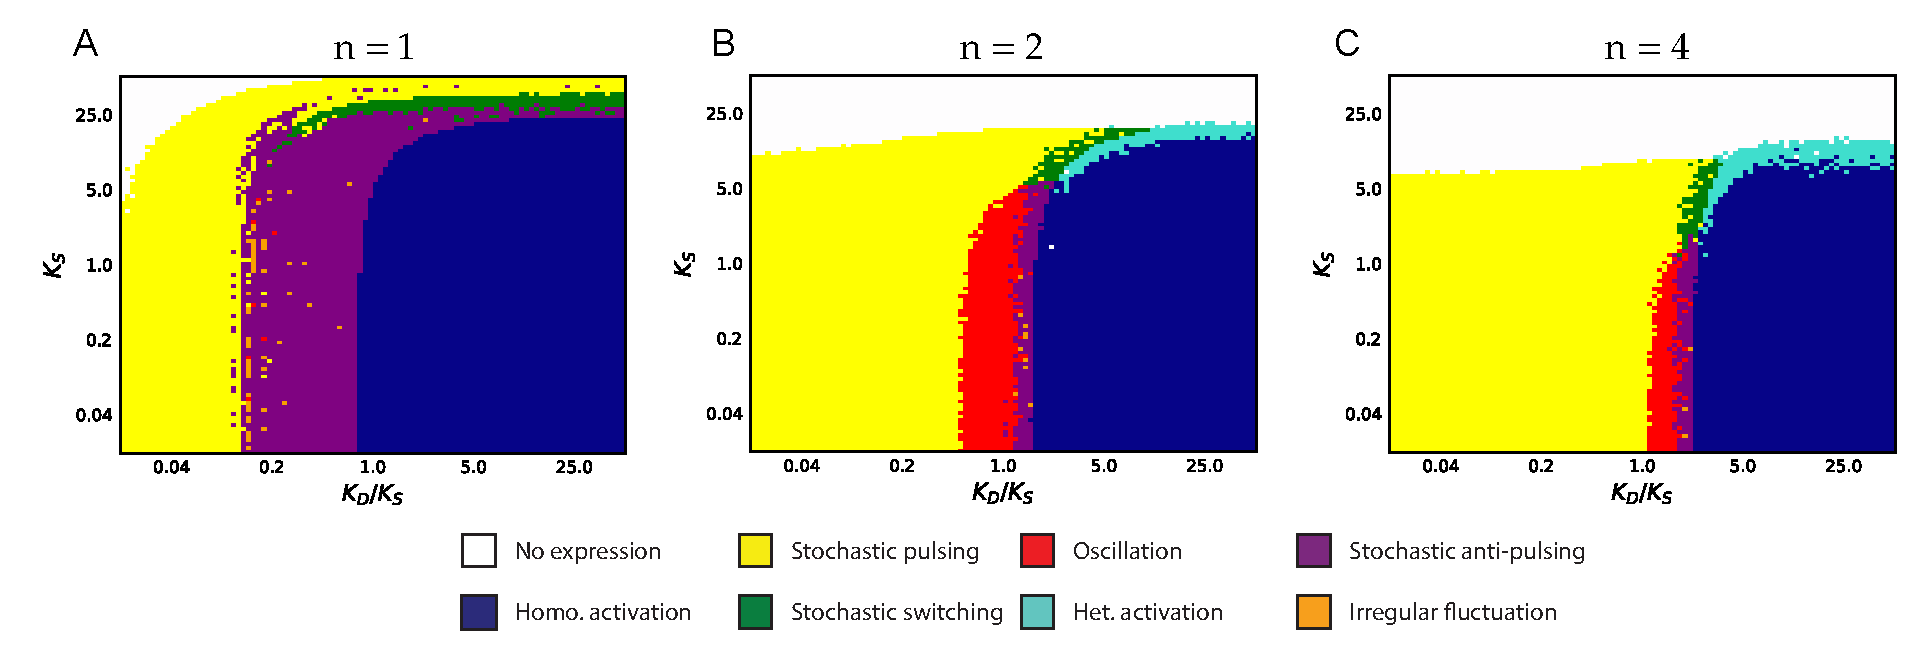
\includegraphics[width = 6in]{behaviour_mappings_diff_n.pdf}
    \caption[
        The mapping of dynamical behaviours across the parametric
        space under different Hill coefficients
        ]{
        \textbf{The mapping of dynamical behaviours across the parametric
        space under different Hill coefficients.} 
        The mathematical model for the alternative sigma factor circuit
        is simulated under three different Hill coefficients
        ($n = 1$, 2 or 4).
        The landscape of the non-ultrasensitive behaviour mapping is
        qualitatively different from the other two.
        $K_S$: the activation threshold (inversely correlated with
        activating strength). $K_D$: the repression threshold (inversely
        correlated with the repressive strength).
    }
    \label{fig:behaviour_mappings_diff_n}
\end{figure}

% why these two behaviours are lost
To explain how some behaviours are lost in the non-ultrasensitive
regime, I examined the non-ultrasensitive counterparts of the
oscillation and stochastic switching dynamics (Figure~
\ref{fig:non_us_counterparts}).
%%
In Figure~\ref{fig:non_us_counterparts},
oscillation (E) and its non-ultrasensitive counterpart (G)
show similar vector fields and the existence of fixed points,
so do stochastic switching (F) and its counterpart (H).
However, their time-dependent trajectories are distinct
from each other.
%%
Under $n = 1$, oscillations collapse into irregular fluctuations,
characterized by no fixed points, but not being periodic either.
%%
Non-ultrasensitivity stochastic switching shows reduced separation
between the ON- and OFF-states and diminished stability of both states.
%%
% Just a possible (intuitive) explanation. Not very confident since no evidence
The lack of ultrasensitivity may promote random walks between
ON- and OFF-states, which makes oscillations and bistability 
difficult to maintain.
%%
% was going to say "intrinsic ultrasensitivity",
% which is a precarious, undefined term
In summary, the loss of ultrasensitivity in the circuit
significantly changes the behaviour mapping across
varying $K_S$ and $K_D$ and makes some behaviours unobtainable.
%%
I showed the importance of ultrasensitivity in maintaining oscillations
and bistability, which is supported by observations of other
genetic circuits \cite{ferrell14c, gardner00c} 
(Section~\ref{sec:biochemical_ultrasensitivity}).
% finally, segue into next section
However, the competition between alternative sigma factors
may be an alternative source of ultrasensitivity that is not accounted 
for in this model of a single sigma factor circuit.

\begin{figure}[ht]
    \centering
    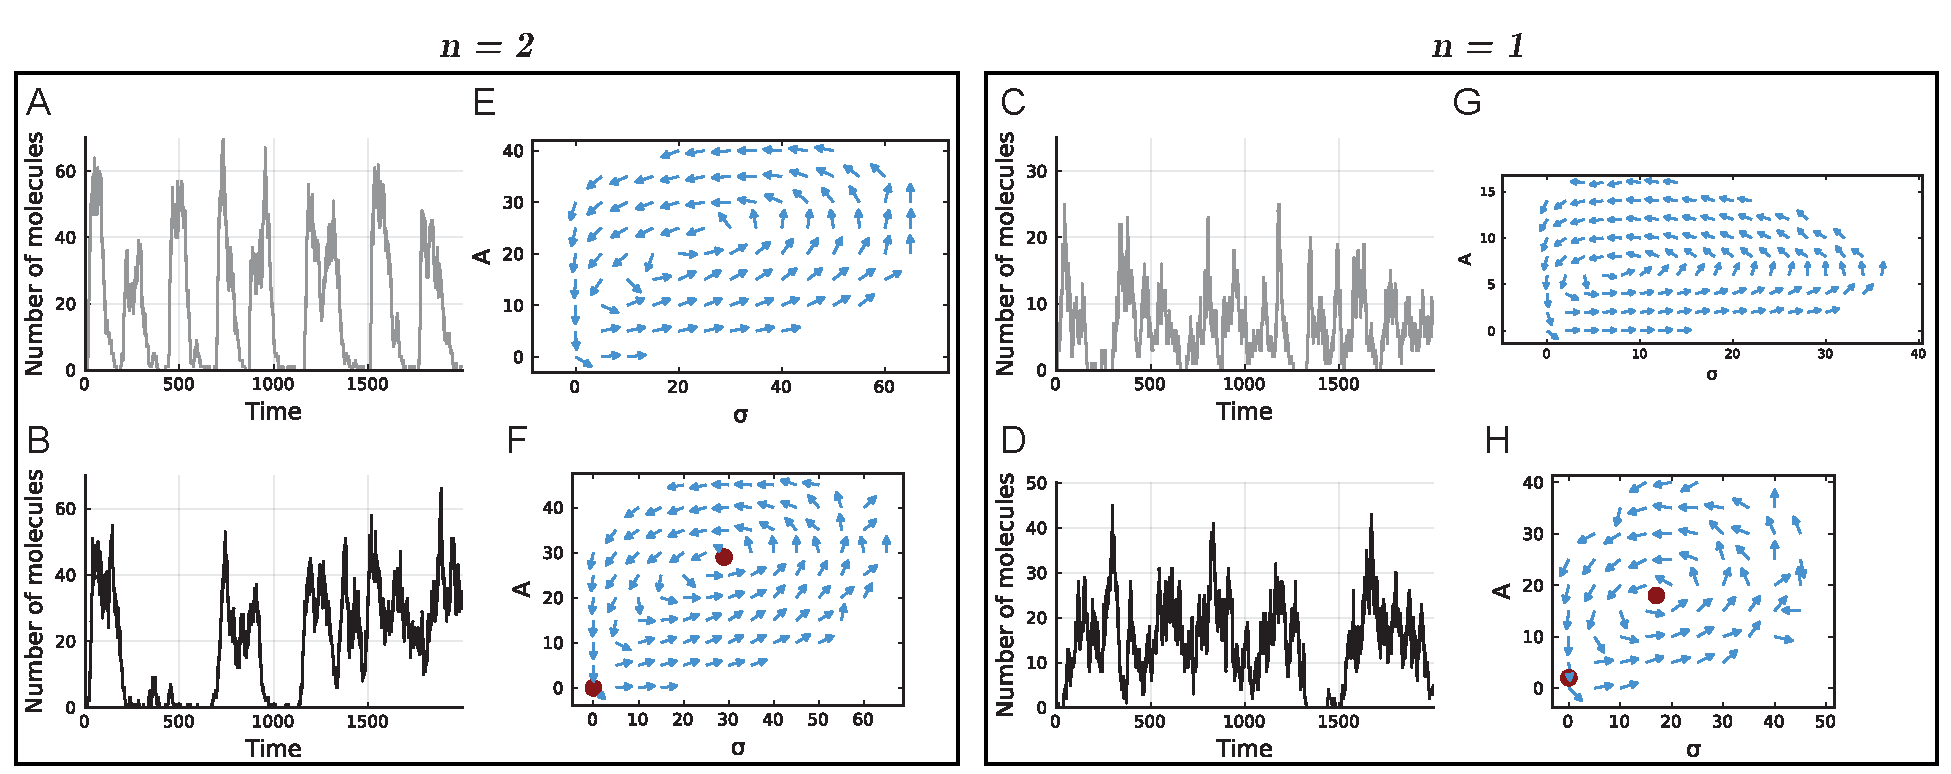
\includegraphics[width = 6in]{non_ultrasensitive_counterparts.pdf}
    \caption[
        The counterparts of oscillation and stochastic switching in 
        non-ultrasensitive regime
        ]{
        \textbf{The counterparts of oscillation and stochastic switching in 
        non-ultrasensitive regime.}
        (A-D) The time-dependent trajectories of 
        oscillation (A) and stochastic switching (B)
        of the ultrasensitive circuit and their counterparts in the
        non-ultrasensitive circuit (C and D).
        The system is exposed to stress at time point 0.
        %%
        (E-H) The corresponding vector field calculated based on
        the trajectories. Red dots mark the fixed points.
        %%
        (A-B and E-F) simulation under $n = 2$, with ultrasensitivity.
        (C-D and G-H) simulation under $n = 1$, without ultrasensitivity.
    }
    \label{fig:non_us_counterparts}
\end{figure}

\clearpage    % some of the figures delay too much
\section{Competition leads to bistability of non-cooperative sigma factor circuit}
\label{sec:competition_to_us}

% why propose new mechanism of ultrasensitivity and how to study it
A previous study shows that \textit{B. subtilis} $\sigma^V$ activates 
heterogeneously upon stress, but there is no known cooperativity 
(thus, also no known source of ultrasensitivity) in the circuit \cite{schwall21a}. 
I have shown that ultrasensitivity is essential for bistable
dynamics, e.g., heterogeneous activation, which suggests that
there could be other source of ultrasensitivity besides binding
cooperativity in the $\sigma^V$ circuit.
Here, I propose new mechanisms (Section~\ref{sec:forced_bistability} and
Section~\ref{sec:both_non_coop_bistability}) 
for the bistability of non-cooperative
alternative sigma factor circuits through the competition of several circuits
for limited RNA polymerase (RNAP) core enzymes.
To validate the mechanisms, I built a mathematical model describing two 
competitive alternative sigma factor circuits and a finite amount of RNAP cores,
where the two sigma factor circuits share the same topology and 
the contribution from the housekeeping sigma factor is reflected by 
the reduced number of RNAP cores (Section~\ref{sec:sigma_competition_model}).

% competitive trajectories show anti-correlations
To visualize the competition between the sigma factors,
I simulated a system of two identical sigma factor circuits, in terms of their
activating/repressive strength and cooperativity, etc., using the
Gillespie algorithm with varying $K_S$ and $K_D$.
The activity of the two sigma factors (in terms of the amount of 
sigma factors bound to the RNAP cores)
show anti-correlations in all of the dynamical behaviours,
including stochastic pulsing, stochastic switching, and activations
(Figure~\ref{fig:time_sharing}).
Depending on the activation threshold ($K_S$), the two sigma factors
can either be activated in parallel (concurrent activation) or the activation 
of one completely repress the other (exclusive activation).
The anti-correlations are important to explain forced bistability
(Section~\ref{sec:forced_bistability}) and,
especially the stochastic switching dynamics here,
represents time sharing activation pattern of the sigma factors,
by which the bacteria may generate heterogeneity in a population 
\cite{schwall21a}.

\begin{figure}[ht]
    \centering
    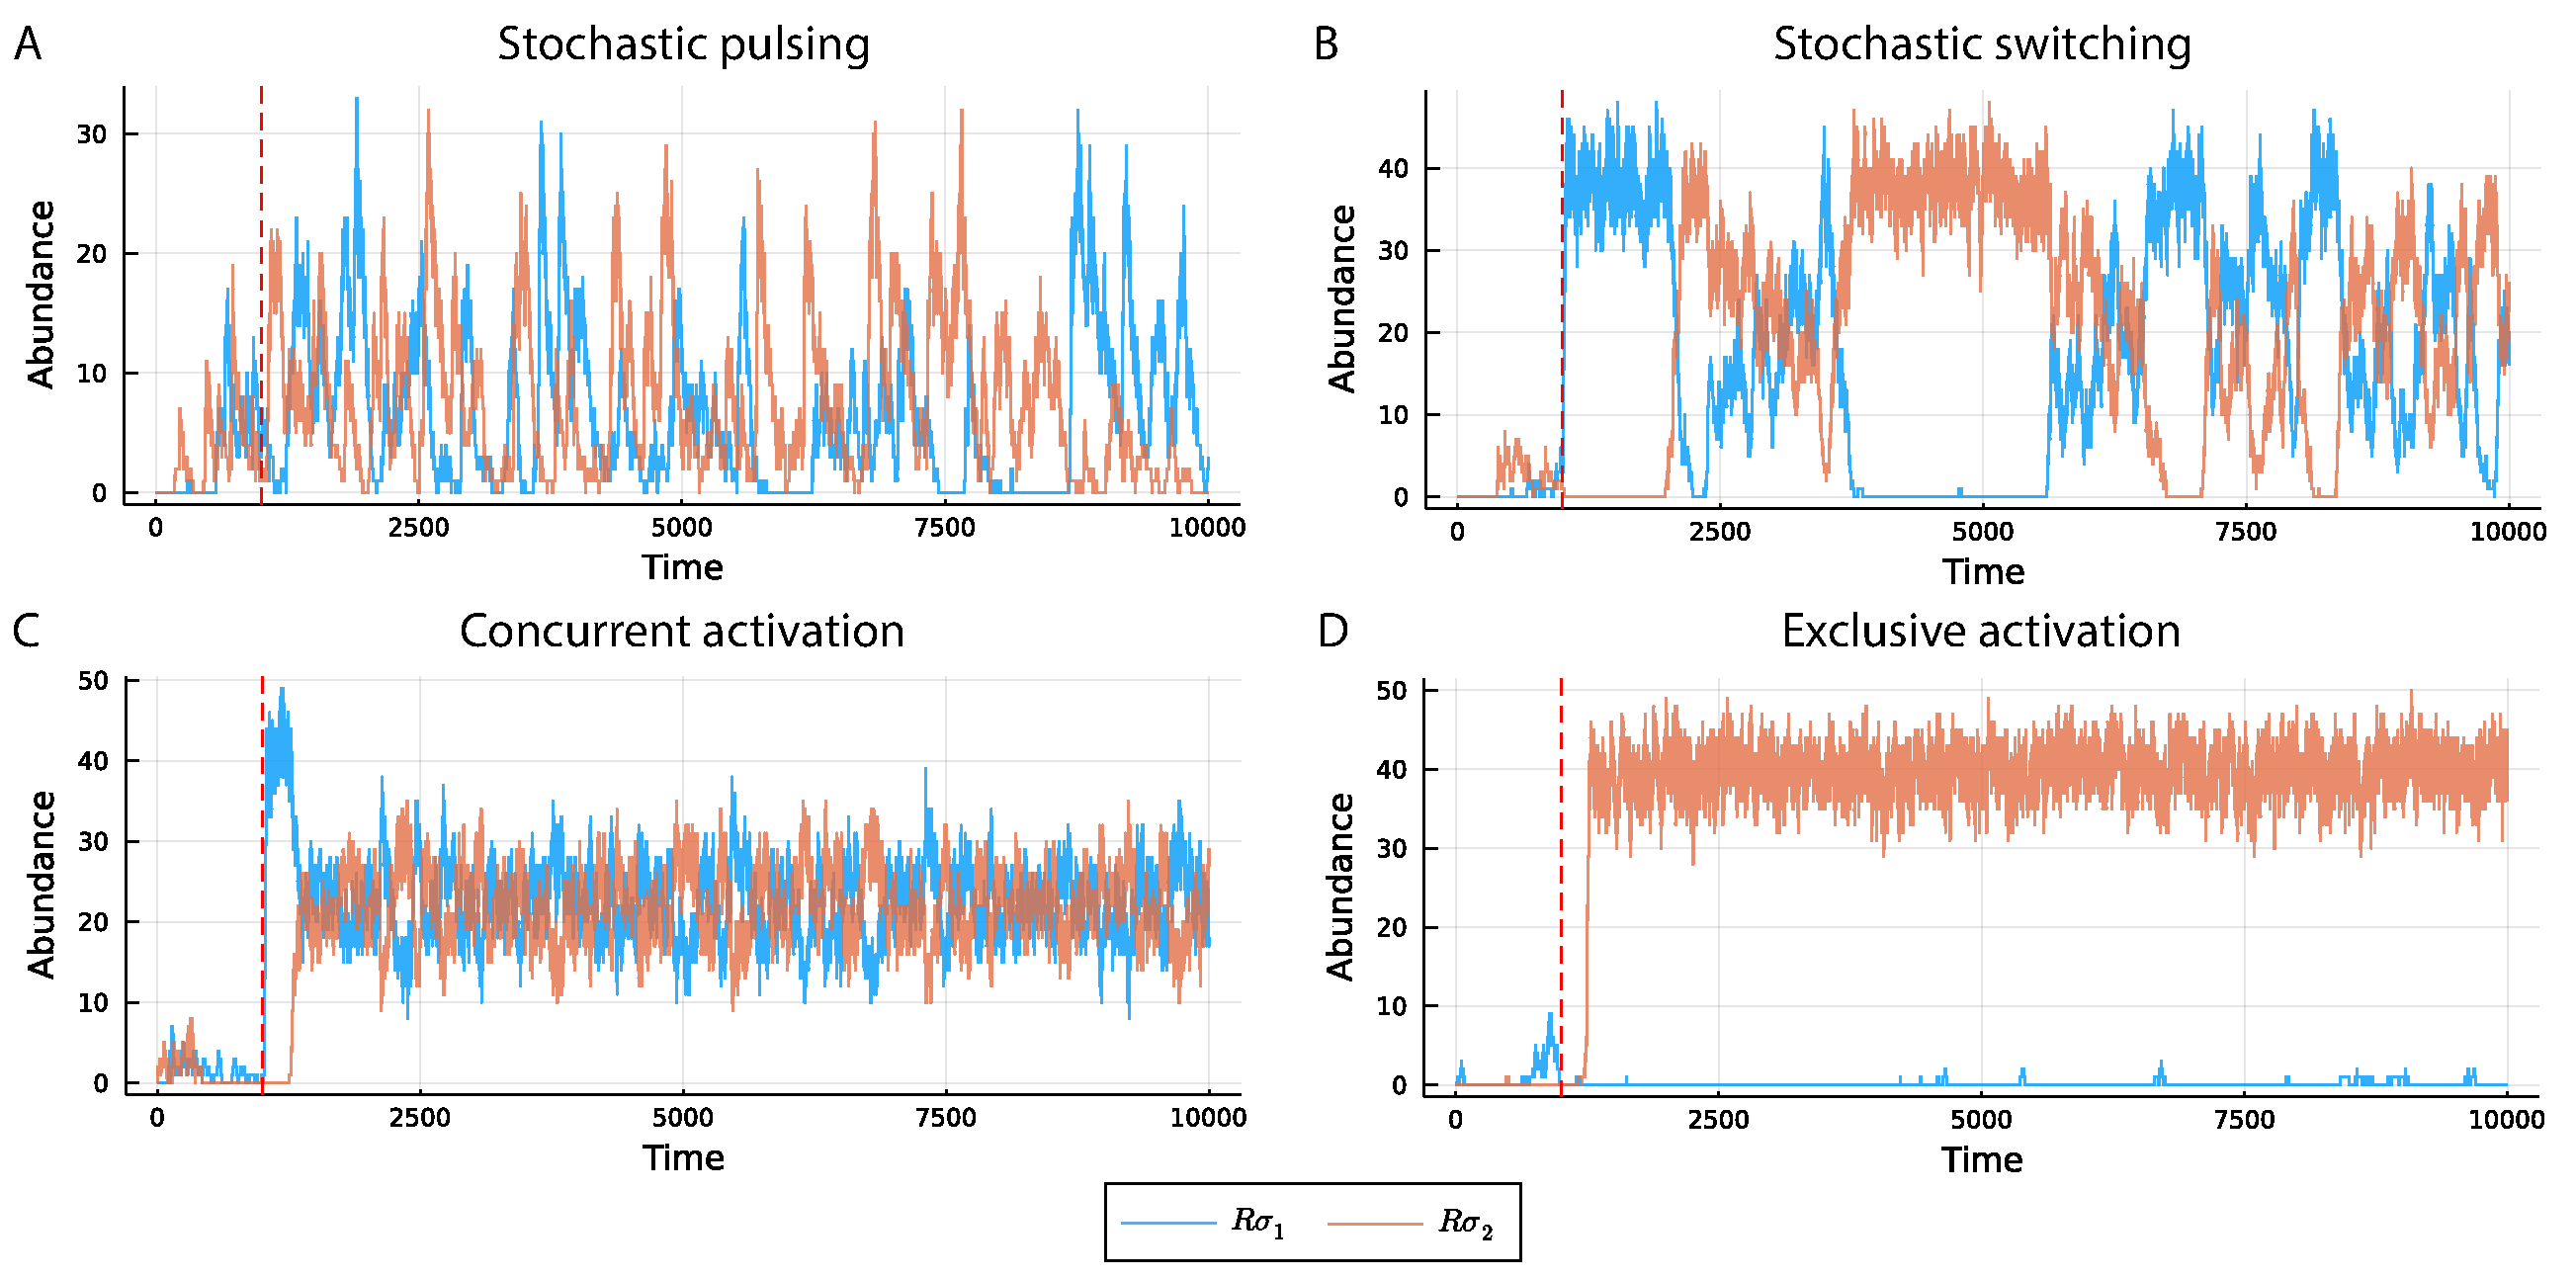
\includegraphics[width = 6in]{time_sharing.pdf}
    \caption[
        Different behaviours of the dual-sigma factor network show
        anti-correlations
        ]{
        \textbf{Different behaviours of the dual-sigma factor network show
        anti-correlations.}
        (A-D) The trajectories of the amount of sigma factors bound
        to the RNAP cores (denoted as $R$), which serves as the activity
        of the sigma factors.
        The total amount of RNAP cores is kept constant at 50.
        The two sigma factor circuits are modelled with the same parameters.
        The red dashed line is the time exposed to stress.
        Binding rate constant between RNAP core and the sigma factor
        $k_1 = 0.005$, the dissociation rate constant
        $k_2 = 0.05$.
    }
    \label{fig:time_sharing}
\end{figure}

\subsection{Forced bistability in asymmetric dual-sigma factor circuits}
\label{sec:forced_bistability}

% forced bistability happens in strong competition
First, I examined a dual-sigma factor competition network where
the Hill coefficients are asymmetric, i.e.,
one of the circuits is without binding cooperativity ($n = 1$, denoted as
$\sigma_1$) while the other one has binding cooperativity
($n = 3$, denoted as $\sigma_2$).
This model represents the actual biochemistry of, e.g., the competition between
\textit{B. subtilis} sigma factors $\sigma^V$ and $\sigma^B$,
since the anti-sigma factor of $\sigma^B$, RsbW, dimerizes and 
cooperatively binds to $\sigma^B$, while the $\sigma^V$ circuit has no known
binding cooperativity \cite{narula16, schwall21a}.
The simulation of the model shows that when the cooperative sigma factor circuit
is in bistable dynamics and when competition is strong,
the non-cooperative sigma factor circuit is forced to be bistable,
while when in weak competition, the dynamics of the cooperative circuit
does not have significant impact on the non-cooperative one
(Figure~\ref{fig:forced_bistability} A).
I suggest that the bistability of $\sigma_2$ causes the amount of free (unbound)
RNAP cores to also switch between high and low states.
Since steady-state expression level of $\sigma_1$ relies on the amount of 
free RNAP cores, it is induced to be bistable.
Unlike $\sigma_2$, the lower state of the non-cooperative $\sigma_1$ bistability
is not necessarily around 0 (Figure~\ref{fig:forced_bistability} B-D).

% forced bistability is stable across k1 and even shows tristability
To ask how the strength of the competition affects the dynamics of the
non-cooperative sigma factor, I simulated the system against different values
of the binding rate constant $k_1$ of $\sigma_1$.
The fixed points are detected as per the classification algorithm
(Section~\ref{sec:classification_algorithm}) and are shown as the 
bifurcation-like diagram (Figure~\ref{fig:forced_bistability} B).
The binding rate constant for the cooperative $\sigma_2$ circuit is fixed.
To keep $\sigma_2$ in bistability, I first examined the region of the
bistable dynamics across the $k_1-K_S$ space (Figure~\ref{fig:k1_KS_mapping}).
Then, the red line is chosen to assign $K_S$ as a linear function of 
$k_1$ across different values of $k_1$ to keep $\sigma_2$ in the bistable regime,
which is $K_S(k_1) = -0.004 \cdot k_1 + 25$.
The bifurcation-like diagram shows that as the hypothetical binding strength
between the sigma factor and the RNAP core increases,
the non-cooperative circuit first transits from the OFF-state to a short
period of bistability, then into tristability (Figure~
\ref{fig:forced_bistability} A middle panel and C).
The tristable dynamics features two non-zero fixed points induced by
the bistable $\sigma_2$ expression and a fixed point at 0 presumably
due to the balance between RNAP holoenzyme formation and sigma
factor degradation (further discussed in Section~\ref{sec:both_non_coop_bistability}).
As $k_1$ of the $\sigma_1$ circuit continues to increase,
the zero fixed point diminishes and the system maintains bistability 
for a rather wide range of parameters.
In summary, in a system of alternative sigma factors competing for a
limited amount RNAP core enzymes, the bistable circuit can force
the non-cooperative circuit to show bistability, or even tristability.

\begin{figure}[ht]
    \centering
    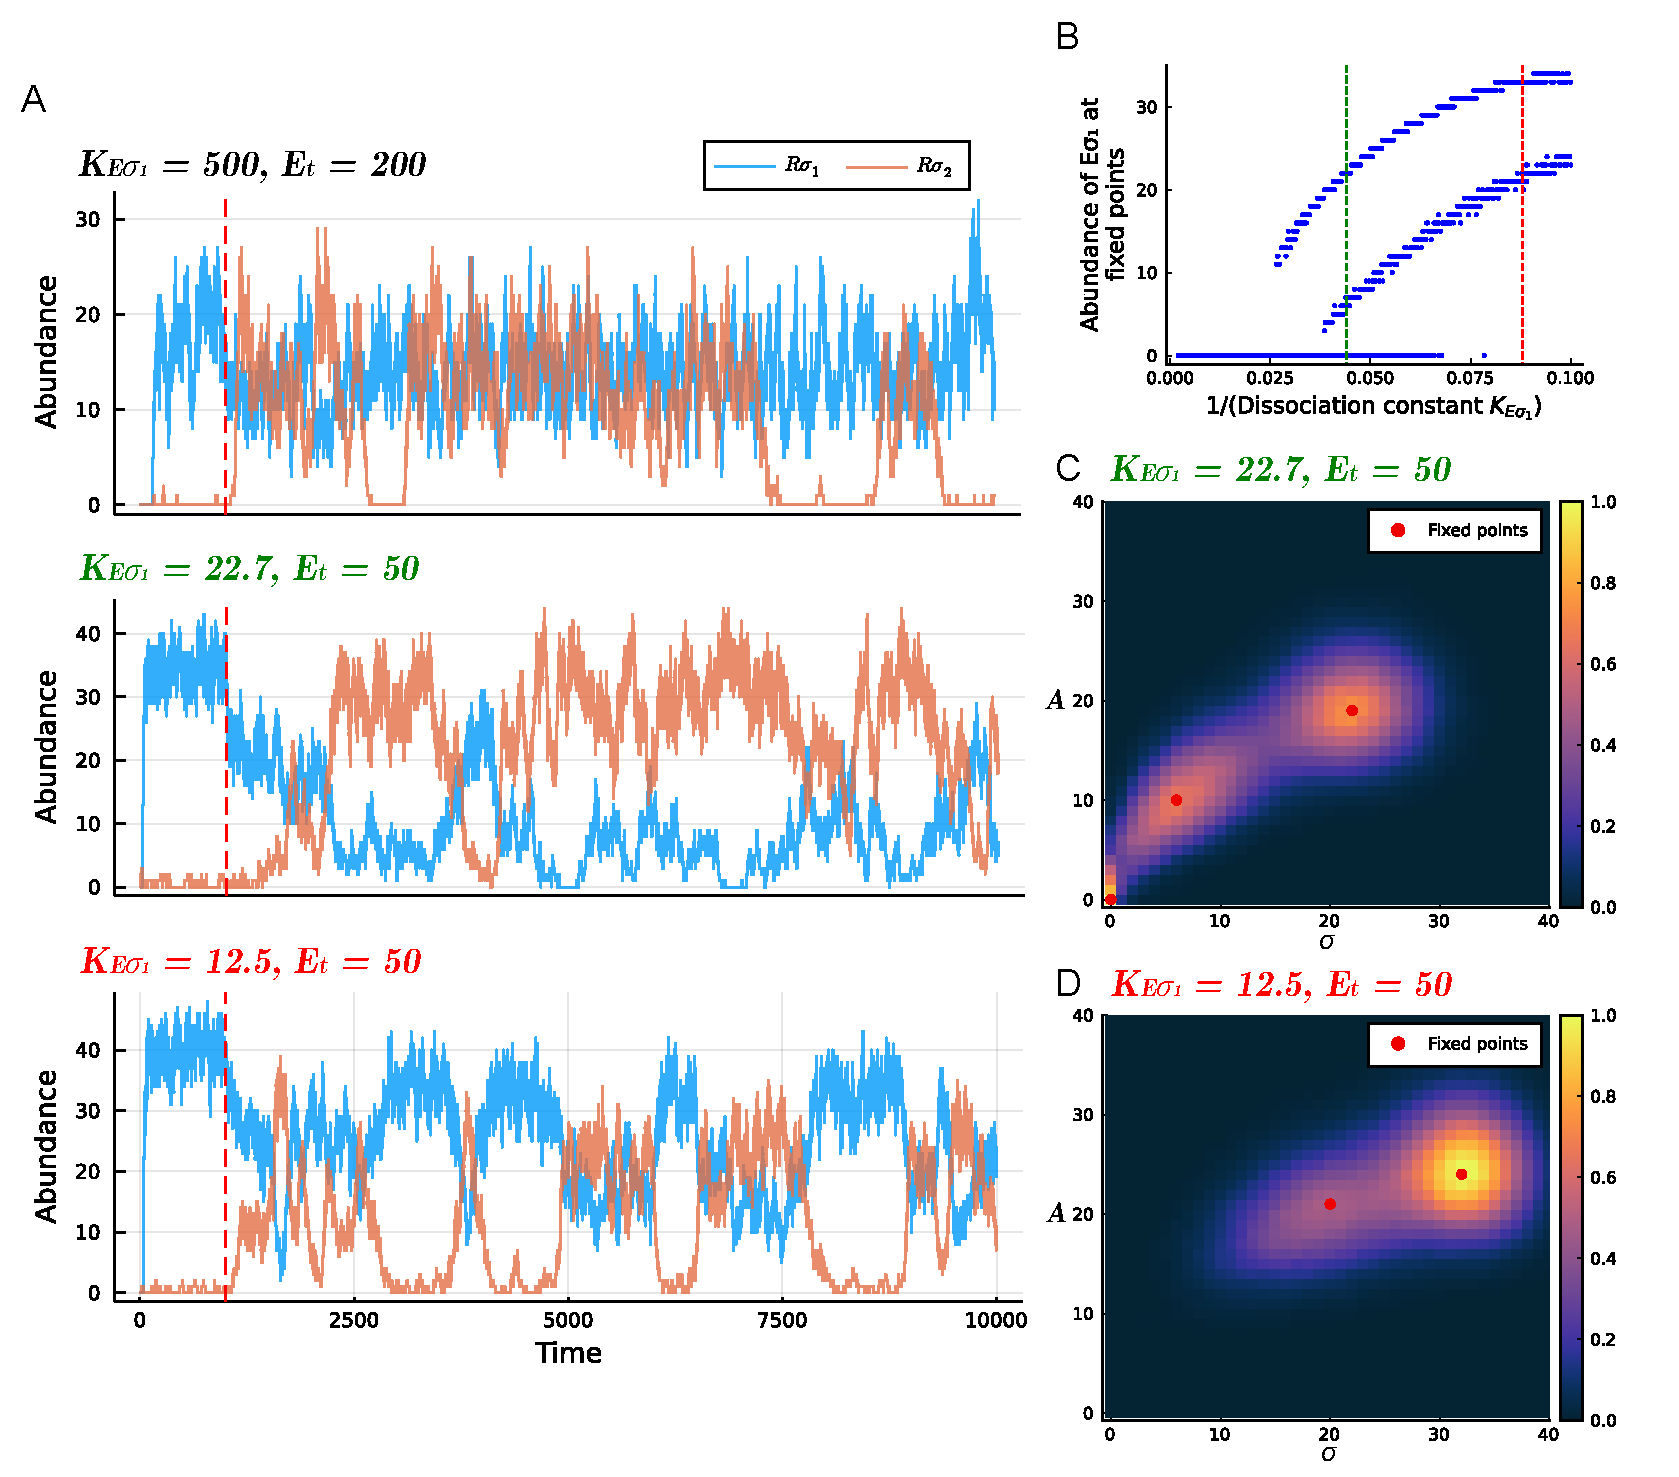
\includegraphics[width = 6in]{forced_bistability.pdf}
    \caption[
        Non-cooperative sigma factor circuit shows forced bistability
        due to the rival bistable circuit
        ]{
        \textbf{Non-cooperative sigma factor circuit shows forced bistability
        due to the rival bistable circuit.}
        (A top) Bistable $\sigma_2$ (cooperative) has no significant 
        influence on the expression of $\sigma_1$ (non-cooperative) under weak
        competition (due to small binding affinity between $\sigma_1$
        and RNAP cores and rather large amount of RNAP cores available).
        (A middle and bottom) the activity of $\sigma_1$ displays forced 
        bistability in strong competition with bistable $\sigma_2$.
        The red dashed line marks exposure to stress.
        $K_{E\sigma_1}$: the dissociation constant of the 
        binding between $\sigma_1$ and the RNAP core ($E$). 
        $E_t$: the total amount of RNAP core enzymes.
        (B) The bifurcation-like diagram of the RNAP core-$\sigma_1$ complex with
        the binding rate constant of $\sigma_1$ as the bifurcation parameter.
        The green and the red dashed line corresponds to the system shown in
        (A middle and C) and (A bottom and D).
        (C-D) The density of the phase paths corresponding to (A middle)
        or (A bottom), respectively showing tristability or bistability.
        $K_{E\sigma_2}$ is fixed at 10 molecules/cell.
    }
    \label{fig:forced_bistability}
\end{figure}

\begin{figure}[ht]
    \centering
    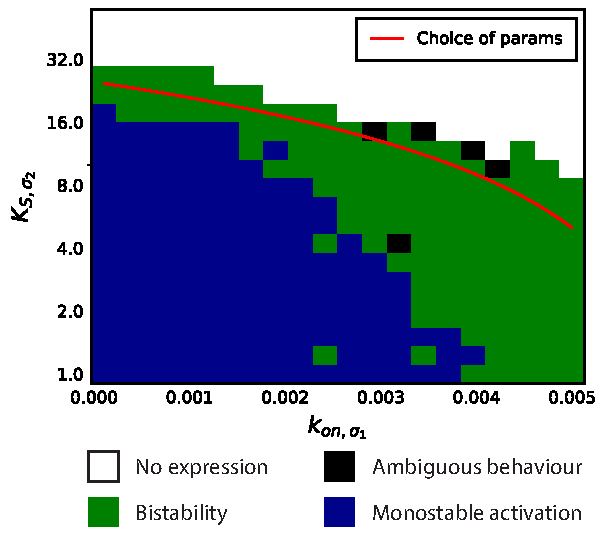
\includegraphics[width = 4in]{k1_KS_mapping.pdf}
    \caption[
        The mapping of the behaviours of non-cooperative sigma 
        factor circuit in the competition model to $k_{on}-K_S$ space
        ]{
        \textbf{The mapping of the behaviours of non-cooperative sigma 
        factor circuit in the competition model to $k_{on}-K_S$ space.}
        The red line shows the function of $K_S$ given $k_{on}$ to keep
        the cooperative sigma factor circuit in bistability, especially,
        $K_S(k_{on}) = -0.004 \cdot k_{on} + 25$.
        $k_{on}$: the binding rate constant of the non-cooperative sigma
        factor. $K_S$: the activation threshold of the cooperative circuit.
    }
    \label{fig:k1_KS_mapping}
\end{figure}

\clearpage
\subsection{Non-cooperative bistability arises from low binding affinity}
\label{sec:both_non_coop_bistability}

Here I explored the situation where none of the sigma factor circuits
in the system are cooperative.
%%
Using the dual-sigma factor competition model with the Hill coefficient
of both circuits set to one, I found a new bistable behaviour with
an almost strict-zero OFF-state and a fluctuating ON-state
(Figure~\ref{fig:strict_zero_bistability} A).
%%
The bistability only holds when (\textit{a}) the amount of available
RNAP cores are limited, and (\textit{b}) the binding affinity between
sigma factors and RNAP cores is considerably low,
%%
e.g., the trajectory in Figure~\ref{fig:strict_zero_bistability} A is 
simulated under $E_t = 50$ and $K_{E\sigma} = 80$
(units: molecules per cell).
%%
In comparison, the binding affinity for the non-ultrasensitive sigma
factor in forced bistability is moderate $K_{E\sigma_1} = 10$
(for parameter specifications see Section~\ref{sec:discussion_parameters}).
%%
The dynamics of the rival sigma factors have no significant effect
on each other (data not shown), which could be the consequence
of low binding affinity.
To reflect this, all simulations that contribute to 
Figure~\ref{fig:strict_zero_bistability} are made with one of the 
sigma circuits turned off.
%%
The density of the occupancy of RNAP cores is clearly bimodal,
with the first peak at zero (silenced) and the second one
around 10\%, which reflects the low binding affinity
(Figure~\ref{fig:strict_zero_bistability} B).
%%
As the relative strength of activating force increases,
the dynamics of the circuit transitions from stochastic switching
to heterogeneous activation (Figure~\ref{fig:strict_zero_bistability} C).
%%
Multiple trajectories in Figure~\ref{fig:strict_zero_bistability} C
simulates a genetically identical bacterial population displaying
heterogeneity in terms of the start of stress response.
%%
Based on the trajectories I plotted the accumulated fraction of
activation in the population.
I found that the variability of
the start of the activation reduces against increasing binding
affinity $K_{E\sigma}$ (Figure~\ref{fig:strict_zero_bistability} D).
%%
Such observation also supports that the weak binding between
sigma factors and RNAP cores accounts for heterogeneous activations.
%%
As the OFF-states feature strict zero-amount of $E\sigma$ complex,
one hypothesis of the mechanism of bistability is that
the low abundance of $E$ and the low affinity of $\sigma$ to it
combined makes the production of a single holoenzyme very rare.
Due to the positive autoregulation of the sigma factor,
the formation of a single holoenzyme can switch on the circuit and
then, it is turned off by random fluctuations.
%%
In summary, I found that in a regime of low RNAP core availability
and low binding affinity of sigma factors to the cores,
sigma factor dynamics exhibits bistability.
This new mechanism may address the activation heterogeneity
of the non-cooperative $\sigma^V$ circuit in \textit{B. subtilis},
and may represent a general mechanism for the generation of 
dynamics that require ultrasensitivity from a non-cooperative circuit.

\begin{figure}
    \centering
    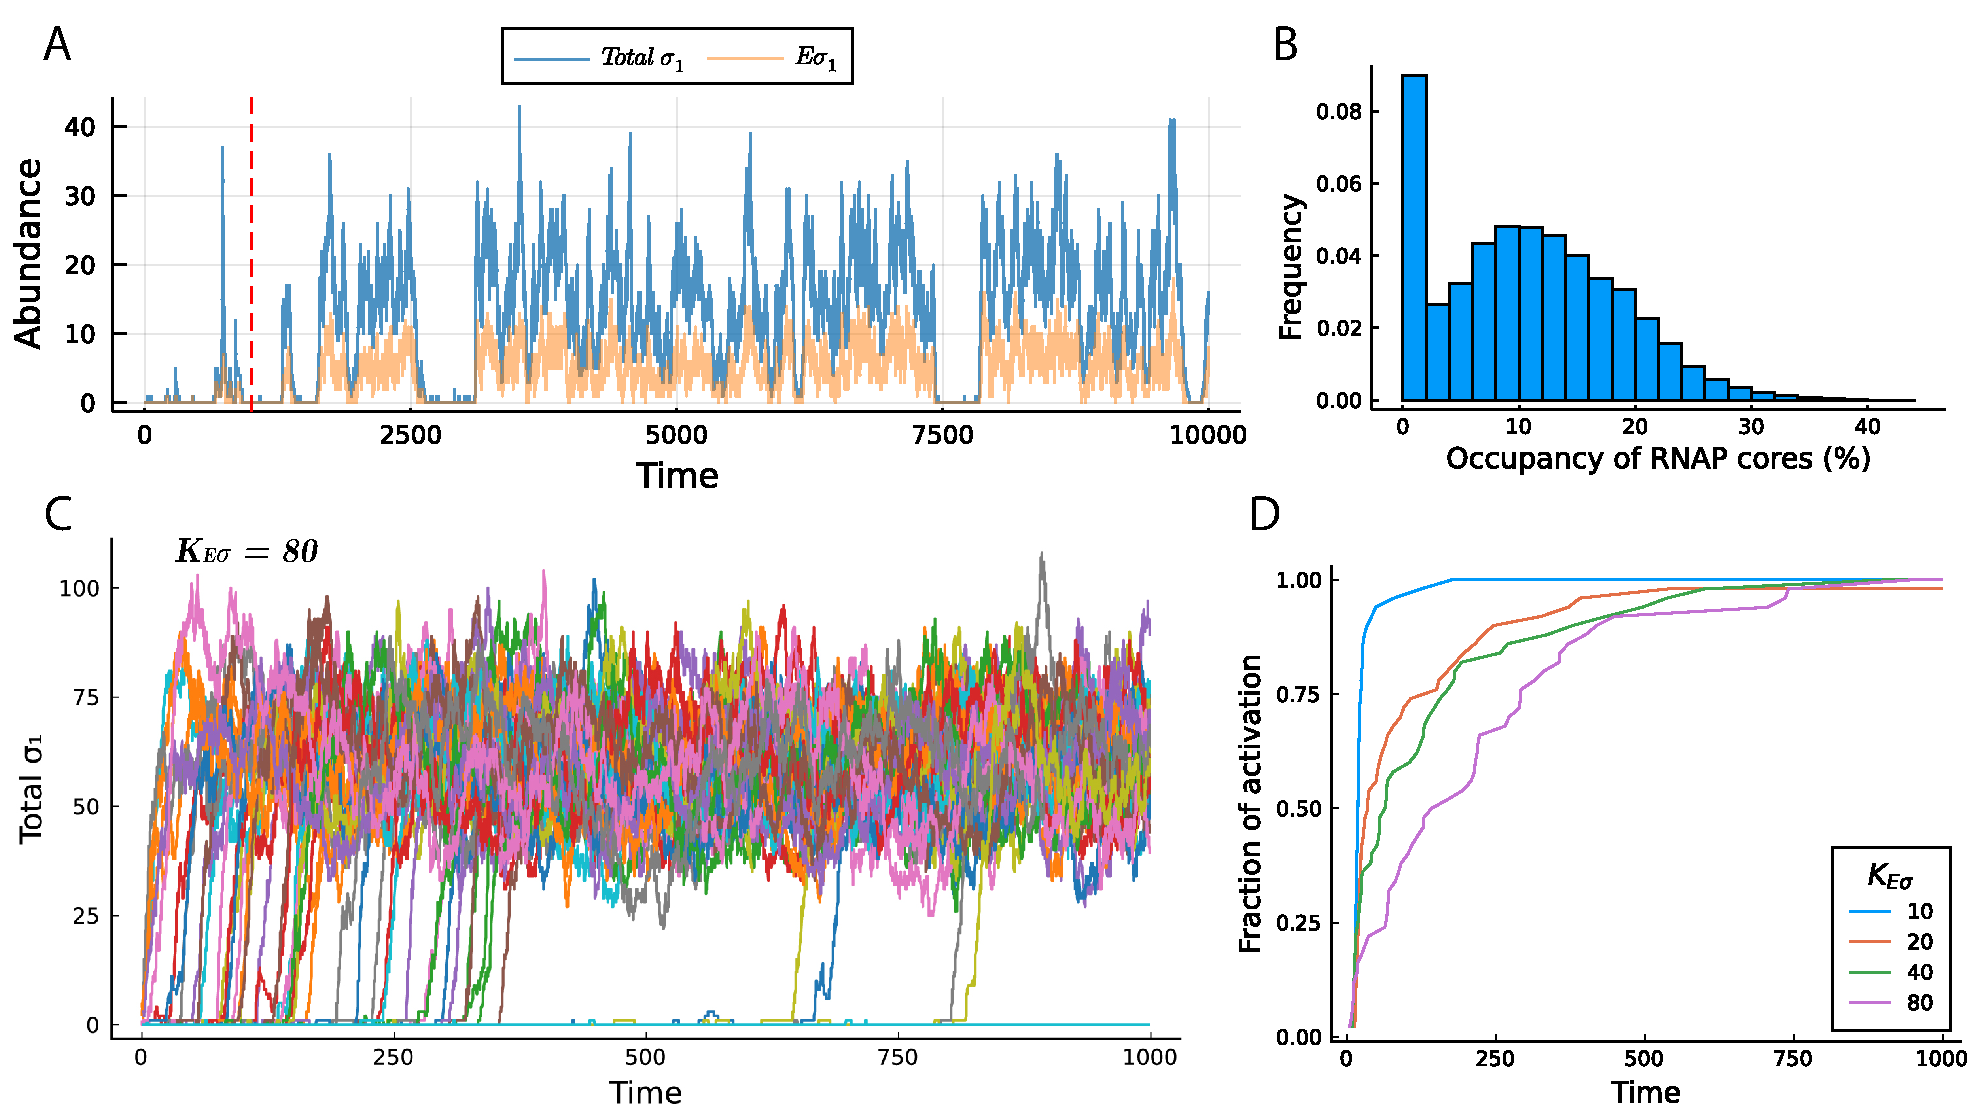
\includegraphics[width = 6in]{strict_zero_bistability.pdf}
    \caption[
        The bistable dynamics of non-cooperative alternative sigma factor
        circuit under low RNAP core affinity
        ]{
        \textbf{The bistable dynamics of non-cooperative alternative sigma factor
        circuit under low RNAP core affinity.}
        (A) Trajectories of total sigma factors and the bound
        sigma factors. The dashed red line indicates exposure to stress.
        In the simulation, $K_{E\sigma} = 80$ and $K_D/K_S = 0.22$.
        (B) Distribution of the occupancy ratio of RNAP cores by sigma factors
        cumulated along the time course of the simulation.
        The distribution is bimodal, which centers at 0 and around 10\%.
        (C) Trajectories of total sigma factors from 50 repeated simulations.
        In the simulation, $K_{E\sigma} = 80$ and $K_D/K_S$ is increased to 0.5
        to stabilize the activation state.
        (D) Accumulated fraction of activation across different binding affinity,
        where activation is defined as the time when
        the amount of sigma factors reaches ON-state.
    }
    \label{fig:strict_zero_bistability}
\end{figure}